\section{Dinámicas factorizables}

En la sección \ref{sec:Ch1PartialTrace} se habló de estados separables como aquellos estados que, descritos por un operador de densidad $\rho\in\densityspace{n}$, tienen la forma
\begin{equation*}
    \rho=\rho_{A}\otimes\rho_{B},
\end{equation*}
donde $\rho_{A}\in\densityspace{m}$, $\rho_{B}\in\densityspace{l}$ y $l+m=n$. Siguiendo esta línea de pensamiento, con \textit{dinámicas factorizables} nos referimos a dinámicas unitarias generadas por Hamiltonianos que no contienen un término de interacción (que en el caso de dos partículas son Hamiltonianos de la forma $\mcH=H_{1}\otimes\Id+\Id\otimes H_{2}$), y que por lo mismo son descritas por operadores $\mcU\in\unitaryspace{n}$ que pueden reescribirse como
\begin{equation*}
    \mcU=U_{A}\otimes U_{B}.
\end{equation*}
Aquí, una vez más, $U_{A}\in\unitaryspace{m}$, $U_{B}\in\unitaryspace{l}$ y $l+m=n$. Los operadores separables están compuestos por operadores que actúan de forma independiente sobre diferentes subsistemas del sistema en custión. En el caso de un sistema compuesto por dos subsistemas de dos niveles, el operador separable está compuesto por dos unitarias que actúan sobre $\hilbert_{2}$. Como el estado de máxima entropía resulta ser separable, las dinámicas separables son una muy buena primera forma de aplicar el formalismo descrito en las secciones anteriores.

Considérese, pues, la aplicación de grano grueso de $n$ a $1$ partículas definida según (\ref{eq:CG}), un estado efectivo $\rho\in\densityspace{2}$ y la aplicación de máxima entropía compatible dada por (\ref{eq:MaxEntAss}). Si la evolución microscópica es factorizable entonces es generada por un Hamiltoniano de la forma
\begin{equation*}
    \mcH=\sum_{k=1}^{n}\omega_{k}\Id_{2^{k-1}}\otimes H_{i} \otimes \Id_{2^{n-k}},
\end{equation*}
siendo la unitaria 
\begin{equation}\label{eq:NFactorUnitaries}
    \mcU_{t}=\Motimes_{k=1}^{n}\text{exp}\qty(-i\omega_{k}H_{k}t)=\Motimes_{k=1}^{n} U_{k}(t)
\end{equation}


\subsection{Caso general}

Si se considera una evolución unitaria de la forma (\ref{eq:NFactorUnitaries}), y se propaga al estado obtenido de la aplicación de máxima entropía, el estado evolucionado toma la forma
\begin{equation*}
    \varrho_{\max}(t)=\Motimes_{k=1}^{n}\frac{1}{Z_{k}}U_{k}(t) e^{\qty(p_{k}\sum_{j}\lambda_{j}\pauli{j})} (U_{k}(t))^{\dag}
\end{equation*}
De esto, el estado efectivo evolucionado obtenido del principio de máxima entropía, en términos de los multiplicadores de Lagrange es
\begin{equation}\label{eq:SeparableEvolution}
    \Gamma_{t}(\rho)=\sum_{k=1}^{n}p_{k} U_{k}(t) \rho_{k} (U_{k}(t))^{\dag}.
\end{equation}
donde hemos denotado $\rho_{k}=\frac{1}{Z_{k}}e^{\qty(p_{k}\sum_{j}\lambda_{j}\pauli{j})}$. 

Por supuesto, esta expresión puede expandirse en términos de exponenciales o de funciones hiperbólicas del vector de Bloch del estado efecivo incial, $\vec{r}_{\rho}$. Si se hace esto para hallar la evolución de un observable $\pauli{i}\in\obspace{2}$ se encuentra que
\begin{equation}\label{eq:SeparableEvolutionExpVal}
    \expval{\pauli{i}(t)}=\frac{1}{2}\sum_{k=1}^{n}p_{k}\tanh(p_{k}\lambda)\Tr[\pauli{i}U_{k}(t) (\hat{r}_{\rho}\cdot\vec{\sigma}) (U_{k}(t))^{\dag}]
\end{equation}

Si se interpreta a la aplicación de grano grueso como en el contexto de la medición de una partícula con probabilidad de error, entoces esperamos que  $p_{1}>\sum_{k=2}^{n}p_{j}$ (o, aún más, $p_{1}\rightarrow 1$). En tal caso, \acnote{Aquí no estuve seguro de qué términos deshechar en la expansión de Taylor}
\begin{align*}
    \expval{\pauli{i}(t)}=&\frac{1}{2}p_{1}\tanh(p_{1}\lambda)\Tr[\pauli{i}U_{1}(t) (\hat{r}_{\rho}\cdot\vec{\sigma}) (U_{1}(t))^{\dag}]+\frac{1}{2}\sum_{k=2}^{n}p_{k}\tanh(p_{k}\lambda)\Tr[\pauli{i}U_{k}(t) (\hat{r}_{\rho}\cdot\vec{\sigma}) (U_{k}(t))^{\dag}]\\
    =_{p_{1}\rightarrow 1}&\frac{1}{2}p_{1}\tanh(p_{1}\lambda)\Tr[\pauli{i}U_{1}(t) (\hat{r}_{\rho}\cdot\vec{\sigma}) (U_{1}(t))^{\dag}]+\frac{1}{2}\lambda p_{k}^{2}\Tr[\pauli{i}U_{k}(t) (\hat{r}_{\rho}\cdot\vec{\sigma}) (U_{k}(t))^{\dag}]
\end{align*}
Reconocemos, pues, dos términos: uno asociado a la evolución esperada de nuestro sistema, descrita por el operador unitario $U_{1}(t)$, y un término de ruido. La acción de este término dependerá tanto de la naturaleza de las evoluciones locales del entorno, como del número de partículas en este.


Por otro lado, en el caso de $n$ partículas idénticas \acnote{No me gusta decirle el caso de las $n$ partículas idéndicas} ($p_{j}=\frac{1}{n}\forall j$), la relación entre la magnitud del vector de Bloch del estado efectivo y los multiplicadores de Lagrange es $\lambda=n\tanh^{-1}(r)$. Esto significa que los observables evolucionan como
\begin{equation*}
    \expval{\pauli{i}(t)}=\frac{1}{2n}\sum_{k=1}^{n}\Tr[\pauli{i}U_{k}(t) (\vec{r}_{\rho}\cdot\vec{\sigma}) (U_{k}(t))^{\dag}].
\end{equation*}
que no es más que una combinación lineal de las mismas componentes evolucionadas de formas diferentes.
\subsection{Ejemplos particulares}

\subsubsection{Dinámica simétrica}

Comenzamos con el caso en el que la dinámica separable simétrica, esto es, de una unitaria $\mcU\in\unitaryspace{2^{n}}$ de la forma
\begin{equation*}
    \mcU_{t}=\Motimes_{k=1}^{n}U(t),
\end{equation*}
donde $U(t)\in\unitaryspace{2}$. Se realiza el mismo proceso: aplicamos la evolución al estado de máxima entropía compatible con un conjunto de observables tomográficamente completos en $\hilbert_{2}$ y propagamos al estado con la unitaria subytacente, para luego pasarlo por la aplicación de grano grueso y recuperar el estado efectivo evolucionado. Este caso es quizá el más sencillo, pues la simetría de la unitaria permite factorizarla:
\begin{align*}
\mcC\qty[\Motimes_{k=1}^{n}U(t) \rho_{k} (U(t))^{\dag}]&=\sum_{k=1}^{n}p_{k} U(t) \rho_{k} (U(t))^{\dag} \\
&=U(t)\qty(\sum_{k=1}^{n}p_{k} \rho_{k}) (U(t))^{\dag}\\
&=U(t)\rho(U^{\dag}(t))^{\dag}.
\end{align*}
La dinámica efectiva tiene la forma
\begin{equation*}
    \Gamma_{t}(\rho)=U(t)\rho(U^{\dag}(t))^{\dag}.
\end{equation*}
Este resultado es natural. No solo no hay interacción entre los diferentes subsistemas, significando esto que no se \textit{filtra} ningún tipo de información entre la partícula de interés y el resto, sino que cada parte evoluciona de manera idéntica: bajo la aplicación de grano grueso, incluso los términos de error arrojan la evolución esperada.

\subsubsection{Entorno invariante}

Centrémonos, momentaneamente, en el régimen $p_{1}>\sum_{k=2}^{n}p_{j}$. Asúmase que la probabilidad de detectar a la $k$-ésima partícula es la misma para todas excepto la primera. Entonces
\begin{equation*}
    p_{k}=\frac{(1-p_{1})}{n-1}\text{ }\forall k\neq 1.
\end{equation*}
El estado de máxima entropía compatible con un estado efectivo $\rho$ tiene la forma
\begin{equation*}
    \varrho_{\max}=\rho_{1}\otimes\qty(\Motimes_{k=2}^{n}\frac{1}{Z_{k}}e^{\frac{(1-p_{1})}{n-1}\sum_{j}\lambda_{j}\pauli{j}})
\end{equation*}
donde, para todo $k$ se cumple que
\begin{equation*}
    \frac{1}{Z_{k}}e^{\frac{1-p_{1}}{n-1}\sum_{j}\lambda_{j}\pauli{j}}=\frac{1}{2}\qty(\Id+\tanh(\frac{1-p_{1}}{n-1}\lambda)\hat{r}_{\rho}\cdot\vec{\sigma})\equiv \rho_{2}.
\end{equation*}
De esto, definimos un entorno efectivo de $n-1$ partículas idénticas según
\begin{equation*}
    \rho_{E}\equiv\rho_{2}^{\otimes(n-1)}.
\end{equation*}
Si el entorno no varía, mientras que el susbsistema de interés se propaga de forma unitaria (esto es, la dinámica subyacente es de la forma $\mcU_{t}=U\otimes\Id_{2^{n-1}}$), entonces la dinámica efectiva es
\begin{equation*}
    \Gamma_{t}(\rho)=p_{1}U(t)\rho_{1}(U(t))^{\dag}+(1-p_{1})\rho_{2}.
\end{equation*}
En términos del vector de Bloch del estado efectivo inicial, denotando $r_{1}=\tan(p_{1}\lambda)$, $r_{2}=\tan((1-p_{1})\lambda)$, y $R$ la rotación generada por $U$:
\begin{equation*}
    r\hat{r}_{\rho}\mapsto p_{1}r_{1}R\hat{r}_{\rho}+(1-p_{1})r_{2}\hat{r}_{\rho}.
\end{equation*}
Esta expresión parece no dar demasiada información: es simplemente la combinación lineal de dos vectores de Bloch, uno que ha sido rotado y otro al que no se le ha hecho nada, pero recordando que el vector de Bloch del estado efectivo inicial cumple $r=p_{1}r_{1}+(1-p_{1})r_{2}$, esta puede ser manipulada para ver que
\begin{equation*}
    r\hat{r}_{\rho}\mapsto R(r\hat{r}_{\rho}-(1-p_{1})r_{2}\hat{r}_{\rho})+(1-p_{1})r_{2}\hat{r}_{\rho}.
\end{equation*}
El resultado es una rotación alrededor de una línea que no pasa por el origen. Una rotación de esta naturaleza puede descomponerse en una rotación a través de un eje que pasa por el origen $R_{0}$ y una traslación $T$ como $T^{-1}\circ R_{0}\circ T$. Nótese que una transformación así no tendría por qué mantener a los estados dentro de la esfera de Bloch, por lo que esta debe depender del estado mismo. 

\begin{figure}[ht!]
    \centering
    \begin{subfigure}{0.32\textwidth}
      \centering
      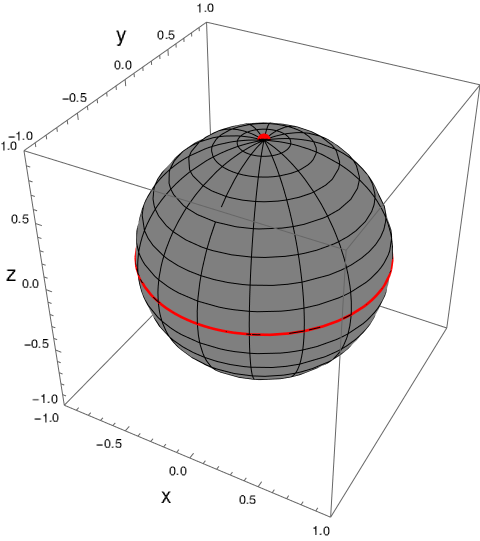
\includegraphics[width=0.9\linewidth]{chapter3/figures_separable/U1xU2_H1=Pi(sz)_H2=Id_z=0.9_p=0.6t=0.png}
      \caption{$t=0.0$}
    \end{subfigure}%
    \begin{subfigure}{0.32\textwidth}
      \centering
      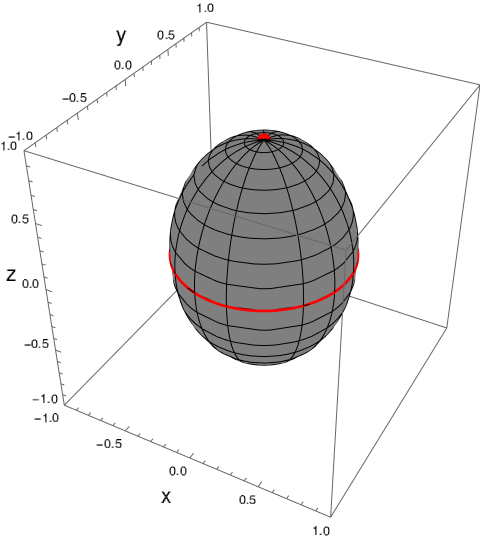
\includegraphics[width=0.9\linewidth]{chapter3/figures_separable/U1xU2_H1=Pi(sz)_H2=Id_z=0.9_p=0.6t=0.25.png}
      \caption{$t=0.25$}
    \end{subfigure}
    \begin{subfigure}{0.32\textwidth}
      \centering
      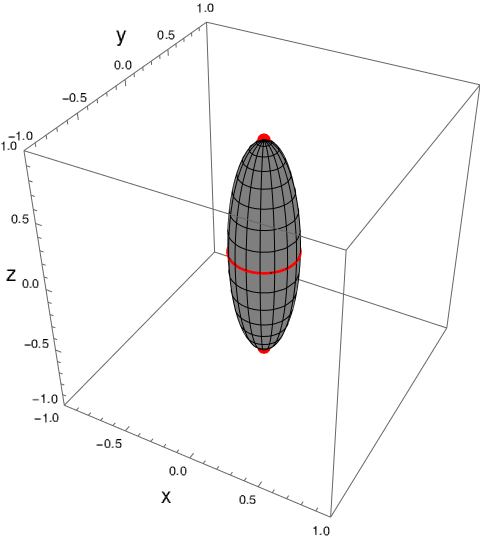
\includegraphics[width=0.9\linewidth]{chapter3/figures_separable/U1xU2_H1=Pi(sz)_H2=Id_z=0.9_p=0.6t=0.5.png}
      \caption{$t=0.5$}
    \end{subfigure}
    \caption{Efecto de la evolución subyacente sobre la esfera de Bloch si $r=0.9$, $p_{1}=0.6$ y $U=e^{-i\pi t \pauli{3}}$. La dramática contracción a lo largo de $z$ se asocia al alto valor de $1-p$.}
    \label{fig:FaseChangeSequence}
\end{figure}

En efecto, la traslación tiene una magnitud $(1-p)r_{B}$ (a notar que la traslación es pequeña, y corresponde al término de ruido) en la dirección opuesta a la del estado (depende del estado tanto en magnitud como en dirección). Así que, aunque esto podría parecer una transformación afín, no lo es, pues depende enteramente del estado. Como tal, la evolución efectiva no es lineal, y no tiene expresión en términos de operadores de Kraus. La figura \ref{fig:FaseChangeSequence} muestra el efecto que una dinámica de este estilo tiene sobre la esfera de Bloch (en particular, el caso $U=e^{-i\omega t \pauli{3}}$). La contracción a lo largo del eje $z$ es un resultado del alto valor de $(1-p_{1})$ (0.4), y no sería visible si $p_{1}\rightarrow 1$.


En efecto, si $p_{1}\approx\frac{1}{2}$, entonces $\rho_{1}\approx\rho_{2}\approx\rho$ y la dinámica efectiva se conviertiría en un canal de desfasamiento:

\begin{align*}
    \Gamma_{\rho}=&p_{1}e^{-i\omega t \pauli{3}}\rho_{1}e^{i\omega t \pauli{3}}+(1-p_{1})\rho_{2}\\
    \approx&\frac{1}{2}(\rho+e^{-i\omega t \pauli{3}}\rho e^{i\omega t \pauli{3}}).
\end{align*}

\subsubsection{Sistema invariante}

Ahora asumamos que es el sistema preferencial el que no evoluciona, mientras que las demás partículas sí lo hacen. Existen diferentes formas de abordar este problema, según la elección de las probabilidades y de la naturaleza de la evolución del entorno. Quizá el caso más sencillo es aquel en el que todas las partículas no preferenciales evolucionan de la misma forma. Esto es, una evolución generada por un Hamiltoniano de la forma
\begin{equation*}
    \mcH=\omega\sum_{k=2}^{n}\Id_{2^{k-1}}\otimes H \otimes \Id_{2^{n-k}}.
\end{equation*}
Por simplicidad, tómese $H=\pauli{3}$. Recordando la ecuación (\ref{eq:rhoArhoB}), se espera que los observables del sistema efectivo evolucionen según
\begin{align*}
    \expval{\pauli{1}(t)}=&p_{1} \expval{\sigma_{1}(0)}_{1}+\sum_{k=2}^{n}p_{k}\Tr[\pauli{1}e^{-it\pauli{3}} \rho_{k} e^{it\pauli{3}}]\\
    \expval{\pauli{2}(t)}=&p_{1} \expval{\sigma_{2}(0)}_{1}+\sum_{k=2}^{n}p_{k}\Tr[\pauli{2}e^{-it\pauli{3}} \rho_{k} e^{it\pauli{3}}]\\
    \expval{\pauli{3}(t)}=&\expval{\pauli{3}(0)},
\end{align*}
que quizá sea más clara escribiéndose en términos de las componentes de los vectores de Bloch de cada partícula (el primer subíndice indica la componente del vector, mientras que el segundo denota la partícula a la que pertenece):
\begin{align*}
    r_{1}(t)=&r_{1,1}(0)+\sum_{k=2}^{n}p_{k}(r_{1,k}\cos(2t)+r_{2,k}\sin(2t))\\
    r_{2}(t)=&r_{2,1}(0)+\sum_{k=2}^{n}p_{k}(r_{2,k}\cos(2t)-r_{1,k}\sin(2t))\\
    r_{3}(t)=&r_{3}(0).
\end{align*}
Esto no es más que la aplicación de la misma rotación sobre todos los vectores de Bloch, a excepción del primero. Reescribiendo,
\begin{align*}
    \vec{r}(t)=&p_{1}\vec{r}_{1}+R_{z}(2t)\vec{r}_{e}\\
    =&\vec{r}(0)+(R_{z}(2t)-\Id)\vec{r}_{e}
\end{align*}
donde $\vec{r}_{e}\sum_{k=2}^{n}p_{k}\vec{r}_{k}$.
En este caso, el primer término es el término invariante, y sería lo único visible en el caso en que el aparato de medición no fallara, mientras que el segundo término corresponde a pequeñas oscilaciones completamente dependientes del estado efectivo inicial. Estas pequeñas oscilaciones son el término de ruido, y por su dependencia en el estado inicial, vuelve a suceder que la evolución no es lineal, y que no tiene representación en términos de operadores de Kraus.

\begin{figure}[ht!]
    \centering
    \begin{subfigure}{0.5\textwidth}
      \centering
      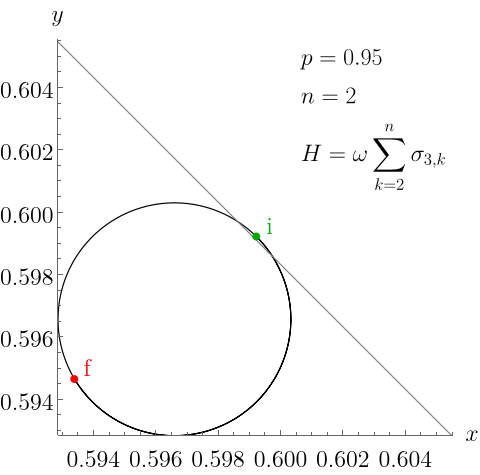
\includegraphics[width=0.9\linewidth]{chapter3/figures_separable/spheretraject_sameHam_difprob_n=2_p=0.95_both.png}
      \caption{Entorno de una partícula.}
    \end{subfigure}%
    \begin{subfigure}{0.5\textwidth}
      \centering
      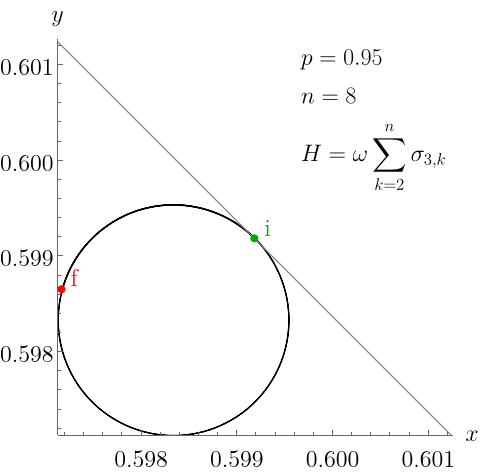
\includegraphics[width=0.9\linewidth]{chapter3/figures_separable/spheretraject_sameHam_difprob_n=8_p=0.95_both.png}
      \caption{Entorno de ocho partículas.}
    \end{subfigure}
    \caption{Oscilaciones periódicas cercanas al valor esperado. La periodicidad no depende de los pesos probabilísticos de cada partícula.}\label{fig:EvolutionOscilations}
\end{figure}


\subsubsection{Cambio de fase con oscilaciones}

Considérese un estado efectivo $\rho\in\densityspace{2}$ de la forma
\begin{equation*}
    \rho(0)=\frac{1}{2}(\Id+r\pauli{3}),
\end{equation*}
asociado a un sistema microscópico de estado $\varrho\in\densityspace{4}$, y que la evolución que experimenta dicho sistema es
\begin{equation*}
    \mcU=e^{-itH_{1}}\otimes e^{-itH_{2}},
\end{equation*}
donde
\begin{align*}
    H_{1}=\pauli{1} & & y & &H_{2}=\frac{\omega}{\sqrt{2}}(\pauli{1}-\pauli{2}).
\end{align*}

El estado de máxima entropía asociado al estado efectivo inicial es el dado por la ecuación (\ref{eq:MaxEntSeparable}). En términos de la catidad observable $r$, y con ayuda de la función $f$ dada por (\ref{eq:r(lambda)}), la evolución del estado de máxima entropía es
\begin{equation*}
    \varrho(t)=\frac{1}{2}\qty(\Id+p\tanh(pf^{-1}(r))\pauli{3}e^{itH_{1}})\otimes\frac{1}{2}\qty(\Id+(p-1)\tanh((p-1)f^{-1}(r))e^{-itH_{2}}\pauli{3}e^{itH_{2}}).
\end{equation*}
El estado efectivo obtenido a través de la aplicación de grano grueso escrita
\begin{align*}
    \rho(t)=&\frac{p}{2}\qty(\Id+p\tanh(pf^{-1}(r))e^{-itH_{1}}\pauli{3}e^{itH_{1}})\\
    &+\frac{(1-p)}{2}\qty(\Id+(p-1)\tanh((p-1)f^{-1}(r))e^{-itH_{2}}\pauli{3}e^{itH_{2}}).
\end{align*}
El valor esperado de $\pauli{3}$, puede hallarse gracias a la ecuación (\ref{eq:SeparableEvolutionExpVal}), siendo particularmente útil la ecuación (\ref{ap:PauliCompExp}) para desarrollar a ambas unitarias. En efecto, estas tienen representación matricial
\begin{align*}
    U_{1}^{t}=\begin{pmatrix}
        \cos(t)+i\sin(t) & 0\\
        0 & \cos(t)-i\sin(t)
    \end{pmatrix}& & y & & U_{2}^{t}=\begin{pmatrix}
        \cos(\omega t) &-\frac{1+i}{\sqrt{2}}\sin(\omega t) \\
        \frac{1-i}{\sqrt{2}}\sin(\omega t) & \cos(\omega t)
    \end{pmatrix}.
\end{align*}
En el caso en que no hubiera error, uno esperaría que el valor esperado de $\pauli{3}$ fuera precisamente $r$ para cualquier tiempo, ya que el cambio en la fase relativa en el primer subsistema no es observable, sin embargo, en este caso se halla que
\begin{equation*}
    \expval{\pauli{3}(t)}=r+(1-p)r_{B}(\cos(2\omega t)-1).
\end{equation*}
\begin{figure}[ht!]
    \centering
    \begin{subfigure}{0.5\textwidth}
      \centering
      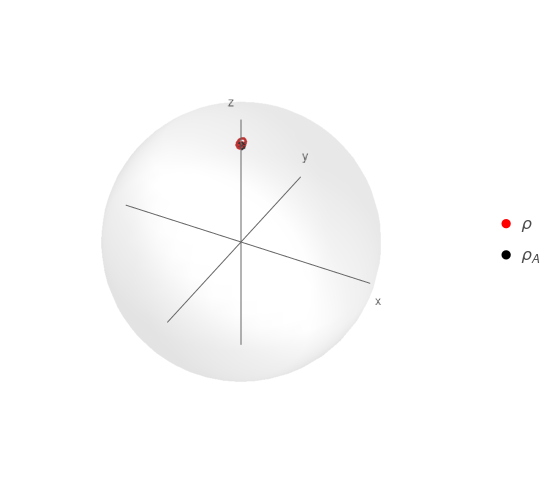
\includegraphics[width=0.9\linewidth]{chapter3/figures_separable/U1xU2_H1=(sz)_H2=15(sx-sy)_z=0.8_p=0.9_far.png}
      \caption{$t=0.0$}
    \end{subfigure}%
    \begin{subfigure}{0.5\textwidth}
      \centering
      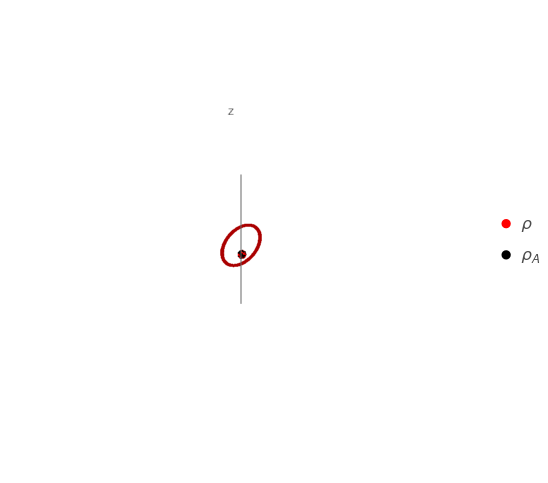
\includegraphics[width=0.9\linewidth]{chapter3/figures_separable/U1xU2_H1=(sz)_H2=15(sx-sy)_z=0.8_p=0.9.png}
      \caption{$t=0.25$}
    \end{subfigure}
    \caption{Oscilaciones cercanas al valor esperado, para cuando $r=r_{z}=0.8$, $p=0.9$ y $\omega=15$. }\label{fig:EvolutionOscilations}
\end{figure}

Este resultado puede observarse en la figura \ref{fig:EvolutionOscilations}, donde se observa que la evolución efectiva se ve como oscilaciones alrededor de un punto cercano al estado del primer subsistema, $\rho_{A}$. Aunque en este caso, el primer subsistema no experimenta cambios, pues es invariante bajo la unitaria $U_{1}$, estas oscilaciones son visibles en casos más generales, como puede observarse en la figura \ref{fig:GeneralOscilations1}.

\begin{figure}[ht!]
    \centering
    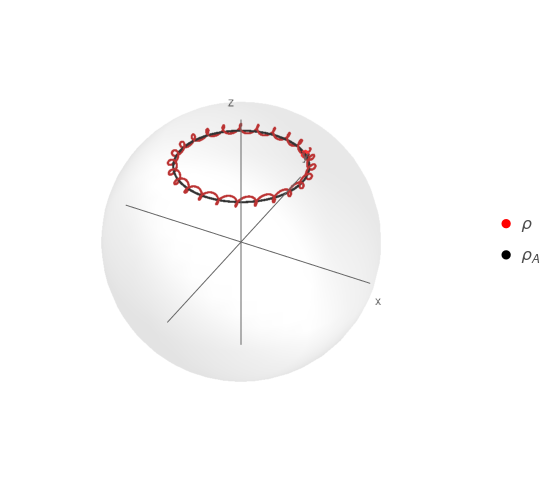
\includegraphics[width=0.6\linewidth]{chapter3/figures_separable/U1xU2_H1=(sz)_H2=15(sx-sy)_z=0.8_p=0.9_wXY=0.5.png}
    \caption{Oscilaciones cercanas al valor esperado. En este caso, el estado inicial no se halla alineado en $z$, por lo que $U_{1}$ lo rota alrededor de dicho eje. Aquí, $r=0.8$ $p=0.9$ y $\omega=15$. }
    \label{fig:GeneralOscilations1}
\end{figure}
